%% Springer Nature single-column manuscript (sn-jnl, "sn-basic" reference style).
%% Same sections and numbers as the other versions: text in ../sections, numbers in ../numbers.tex.
\documentclass[pdflatex,sn-basic]{sn-jnl}

\usepackage{graphicx}
\usepackage{multirow}
\usepackage{amsmath,amssymb,amsfonts}
\usepackage{amsthm}
\usepackage{mathrsfs}
\usepackage{xcolor}
\usepackage{textcomp}
\usepackage{manyfoot}
\usepackage{booktabs}
\usepackage{algorithm}
\usepackage[hyphens]{xurl}

\graphicspath{{../../docs/figures/}}
% GENERATED by `python -m src.report.paper_numbers`. Do not edit: change the freeze and regenerate.
% source: benchmarks/results_freeze_v5.json  sha256 4ada25e3b5a99a4b  frozen_at 2026-10-21T11:19:28.292835+00:00  values 109
\providecommand{\fzLegsTotal}{26{,}369} % legs_total (legs)
\providecommand{\fzCorridorsTotal}{2{,}783} % corridors_total (corridors)
\providecommand{\fzMedianGapRatio}{2} % median_gap_ratio (x)
\providecommand{\fzCorridorsTested}{1{,}130} % corridors_tested (corridors)
\providecommand{\fzBottlenecks}{273} % bottlenecks (corridors)
\providecommand{\fzFasterCorridors}{512} % faster_corridors (corridors)
\providecommand{\fzLegsCovered}{20{,}739} % legs_covered (legs)
\providecommand{\fzRobustnessBottlenecks}{34} % robustness_bottlenecks (corridors)
\providecommand{\fzSplitTrain}{21{,}095} % split_train (legs)
\providecommand{\fzSplitTest}{5{,}274} % split_test (legs)
\providecommand{\fzPctDelayed}{49.69} % pct_delayed (%)
\providecommand{\fzMaeOsrm}{107.09} % mae_osrm (min)
\providecommand{\fzMaeCorridorMean}{36.13} % mae_corridor_mean (min)
\providecommand{\fzChampionModel}{random\_forest} % champion_model (text)
\providecommand{\fzMaeChampion}{36.89} % mae_champion (min)
\providecommand{\fzCorridorsImproved}{1{,}369} % corridors_improved (corridors)
\providecommand{\fzDocAgentFOneVOne}{0.853} % doc_agent_f1_v1 (text)
\providecommand{\fzDocAgentFOneVTwo}{0.929} % doc_agent_f1_v2 (text)
\providecommand{\fzStreamIdentical}{500} % stream_identical (of 500)
\providecommand{\fzStreamEvents}{52{,}738} % stream_events (events)
\providecommand{\fzStreamProducedEps}{886.4} % stream_produced_eps (events/sec)
\providecommand{\fzStreamScoringEps}{739.9} % stream_scoring_eps (events/sec)
\providecommand{\fzStreamLatencyPFiveZeroS}{28.9} % stream_latency_p50_s (s)
\providecommand{\fzOrderEvalRun}{50} % order_eval_run (of 50)
\providecommand{\fzOrderEvalSuccess}{1} % order_eval_success (text)
\providecommand{\fzOrderEvalInvented}{0} % order_eval_invented (orders)
\providecommand{\fzLifecycleCases}{10} % lifecycle_cases (cases)
\providecommand{\fzLifecycleBooked}{5} % lifecycle_booked (cases)
\providecommand{\fzLifecycleTicketed}{2} % lifecycle_ticketed (cases)
\providecommand{\fzInvoiceCases}{20} % invoice_cases (invoices)
\providecommand{\fzInvoiceCorrect}{20} % invoice_correct (invoices)
\providecommand{\fzMedianBarMae}{33.04} % median_bar_mae (min)
\providecommand{\fzModelVTwoMae}{30.9} % model_v2_mae (min)
\providecommand{\fzDocExtractionAccuracy}{0.9786} % doc_extraction_accuracy (share)
\providecommand{\fzDocExtractionRows}{20} % doc_extraction_rows (rows)
\providecommand{\fzAssistantRouteAccuracy}{0.9} % assistant_route_accuracy (share)
\providecommand{\fzScaleRows}{56{,}353{,}613} % scale_rows (rows)
\providecommand{\fzExceptionPrecisionAsOf}{0.5855} % exception_precision_as_of (share)
\providecommand{\fzAssistantGroundedness}{0.9444} % assistant_groundedness (share)
\providecommand{\fzKafkaFileAlertsIdentical}{true} % kafka_file_alerts_identical (bool)
\providecommand{\fzAdoptedStreamEqualsBatch}{500} % adopted_stream_equals_batch (legs)
\providecommand{\fzFreshCloneRebuildS}{4{,}258} % fresh_clone_rebuild_s (seconds)
\providecommand{\fzOrderEvalScaleHeldout}{0.85} % order_eval_scale_heldout (share)
\providecommand{\fzOrderEvalScaleAdversarialHeldout}{0.7} % order_eval_scale_adversarial_heldout (share)
\providecommand{\fzOrderEvalScaleCases}{200} % order_eval_scale_cases (cases)
\providecommand{\fzInvoiceEvalScaleAccuracy}{0.9} % invoice_eval_scale_accuracy (share)
\providecommand{\fzInvoiceEvalScaleCases}{200} % invoice_eval_scale_cases (invoices)
\providecommand{\fzInvoiceEvalScaleFalseDisputes}{0} % invoice_eval_scale_false_disputes (invoices)
\providecommand{\fzLifecycleEvalScalePaths}{3} % lifecycle_eval_scale_paths (of 3)
\providecommand{\fzLifecycleEvalScaleRouting}{1} % lifecycle_eval_scale_routing (share)
\providecommand{\fzLifecycleEvalScaleCases}{100} % lifecycle_eval_scale_cases (lifecycles)
\providecommand{\fzBarOldMedianMae}{33.0423} % bar_old_median_mae (min)
\providecommand{\fzBarBackoffMae}{32.3932} % bar_backoff_mae (min)
\providecommand{\fzBarShrunkMae}{32.9221} % bar_shrunk_mae (min)
\providecommand{\fzBarBackoffValidationMae}{29.3567} % bar_backoff_validation_mae (min)
\providecommand{\fzColdLegsTest}{204} % cold_legs_test (legs)
\providecommand{\fzColdMaeBackoff}{132.9706} % cold_mae_backoff (min)
\providecommand{\fzColdMaeModel}{100.1619} % cold_mae_model (min)
\providecommand{\fzWarmMaeBackoff}{28.3464} % warm_mae_backoff (min)
\providecommand{\fzWarmMaeModel}{28.1182} % warm_mae_model (min)
\providecommand{\fzVThreeValidationMae}{31.1425} % v3_validation_mae (min)
\providecommand{\fzVTwoValidationMae}{30.17} % v2_validation_mae (min)
\providecommand{\fzVThreeTestMae}{31.4032} % v3_test_mae (min)
\providecommand{\fzServedVsBarDelta}{-1.4884} % served_vs_bar_delta (min)
\providecommand{\fzServedVsBarCiLow}{-2.2465} % served_vs_bar_ci_low (min)
\providecommand{\fzServedVsBarCiHigh}{-0.738} % served_vs_bar_ci_high (min)
\providecommand{\fzServedMaeCiLow}{29.0171} % served_mae_ci_low (min)
\providecommand{\fzServedMaeCiHigh}{32.6355} % served_mae_ci_high (min)
\providecommand{\fzAuditRobustHeadlineSlower}{0} % audit_robust_headline_slower (corridors)
\providecommand{\fzAuditRobustHeadlineFaster}{0} % audit_robust_headline_faster (corridors)
\providecommand{\fzAuditByWelchSlower}{218} % audit_by_welch_slower (corridors)
\providecommand{\fzAuditPlaceboRejection}{0.6387} % audit_placebo_rejection (share)
\providecommand{\fzAuditPlaceboDiscoveries}{680.205} % audit_placebo_discoveries (corridors)
\providecommand{\fzEbThresholdLog}{1.1838} % eb_threshold_log (log)
\providecommand{\fzEbTopTwoZeroJaccardRaw}{0.1012} % eb_top20_jaccard_raw (jaccard)
\providecommand{\fzEbTopTwoZeroJaccardEb}{0.1502} % eb_top20_jaccard_eb (jaccard)
\providecommand{\fzStabilityUniverse}{807} % stability_universe (corridors)
\providecommand{\fzStabilityJaccard}{0.6364} % stability_jaccard (jaccard)
\providecommand{\fzStabilitySpearman}{0.9084} % stability_spearman (rho)
\providecommand{\fzStabilityStillSlower}{0.9769} % stability_still_slower (share)
\providecommand{\fzStabilityBaseRate}{0.3978} % stability_base_rate (share)
\providecommand{\fzReportedMae}{29.6578} % reported_mae (min)
\providecommand{\fzReportedMaeCiLow}{27.8611} % reported_mae_ci_low (min)
\providecommand{\fzReportedMaeCiHigh}{31.1193} % reported_mae_ci_high (min)
\providecommand{\fzReportedVsBarDelta}{-2.7354} % reported_vs_bar_delta (min)
\providecommand{\fzReportedVsBarCiLow}{-3.4132} % reported_vs_bar_ci_low (min)
\providecommand{\fzReportedVsBarCiHigh}{-2.107} % reported_vs_bar_ci_high (min)
\providecommand{\fzReportedValidationMae}{27.2368} % reported_validation_mae (min)
\providecommand{\fzZooLightgbmHuberMae}{30.5347} % zoo_lightgbm_huber_mae (min)
\providecommand{\fzZooXgboostMae}{29.7104} % zoo_xgboost_mae (min)
\providecommand{\fzZooHistgbrMae}{29.7456} % zoo_histgbr_mae (min)
\providecommand{\fzZooLinearMae}{33.9563} % zoo_linear_mae (min)
\providecommand{\fzExcPrecisionAsOfRate}{0.5855} % exc_precision_as_of_rate (share)
\providecommand{\fzExcPrecisionCiLow}{0.562} % exc_precision_ci_low (share)
\providecommand{\fzExcPrecisionCiHigh}{0.6085} % exc_precision_ci_high (share)
\providecommand{\fzExcAlerts}{1{,}720} % exc_alerts (legs)
\providecommand{\fzExcGainPoints}{4.45} % exc_gain_points (points)
\providecommand{\fzExcGainCiLow}{0.0353} % exc_gain_ci_low (share)
\providecommand{\fzExcGainCiHigh}{0.0538} % exc_gain_ci_high (share)
\providecommand{\fzExcGainZ}{9.8904} % exc_gain_z (z)
\providecommand{\fzAblationOrderCases}{18} % ablation_order_cases (cases)
\providecommand{\fzAblationOrderLlmAccuracy}{0.8778} % ablation_order_llm_accuracy (share)
\providecommand{\fzAblationOrderLlmCiLow}{0.7943} % ablation_order_llm_ci_low (share)
\providecommand{\fzAblationOrderLlmCiHigh}{0.9304} % ablation_order_llm_ci_high (share)
\providecommand{\fzAblationOrderUnanimity}{0.8333} % ablation_order_unanimity (share)
\providecommand{\fzAblationOrderKappa}{0.82} % ablation_order_kappa (kappa)
\providecommand{\fzHardOrderRules}{0.7} % hard_order_rules (share)
\providecommand{\fzHardOrderCases}{100} % hard_order_cases (cases)
\providecommand{\fzHardInvoiceRules}{1} % hard_invoice_rules (share)

\newif\ifjournal \journaltrue
\newcommand{\streamsec}{(Section~\ref{sec:stream})}

% Mentor details (the affiliation below is shared with the student authors).
\newcommand{\mentorgiven}{Anshi}
\newcommand{\mentorsurname}{Bajaj}
\newcommand{\mentoremail}{anshi.bajaj@nmims.edu}

\begin{document}

\title[Localising Route-Estimate Error in Road Freight]{Localising Systematic Route-Estimate Error in Road Freight: Dependence-Aware Corridor Auditing, Residual Prediction and a Measured Agent Layer}

\author*[1]{\fnm{Kuchuru Sai Krishna} \sur{Reddy}}\email{kuchurusaikrishnareddy@gmail.com}
\equalcont{These authors contributed equally to this work.}

\author[1]{\fnm{Makkena} \sur{Lahari}}\email{laharisuresh6666@gmail.com}
\equalcont{These authors contributed equally to this work.}

\author[1]{\fnm{Shery Mounika} \sur{Reddy}}\email{sherymounikareddy.2006@gmail.com}
\equalcont{These authors contributed equally to this work.}

\author[1]{\fnm{\mentorgiven} \sur{\mentorsurname}}\email{\mentoremail}

\affil*[1]{\orgdiv{Department of Computer Science and Data Science}, \orgname{SVKM's Narsee Monjee Institute of Management Studies}, \city{Hyderabad}, \country{India}}

\abstract{Road-freight operators schedule against route-planner estimates, and the OSRM estimate recorded in Delhivery's public trip data runs short almost every time: \fzLegsTotal{} legs, the median taking \fzMedianGapRatioDpOne{} times the estimate. We ask where this error concentrates and how confidently that can be said. A Welch audit with false-discovery control flags \fzBottlenecks{} corridors as slower than the network, but legs of one recurring service are correlated (design effect about \fzDepDesignEffectMedianDpOne{}), and on placebo data with meaningless corridor labels the same procedure returns about \fzAuditPlaceboDiscoveriesDpOne{} discoveries; a cluster-aware permutation test confirms \fzAuditRobustHeadlineSlower{} corridors at its pre-registered strictness. Corridor effects nonetheless persist between halves of the period (rank correlation \fzStabilitySpearmanDpTwo{}), and empirical-Bayes ranking is only slightly more stable across support floors than raw ranking. For prediction, a gradient-boosted residual over a hierarchical back-off baseline, whose cold-start fallback is fair, reaches \fzReportedMaeDpTwo{} minutes MAE against the baseline's \fzBarBackoffMaeDpTwo{} (difference \fzReportedVsBarDeltaDpTwo{}, day-block 95\% interval [\fzReportedVsBarCiLowDpTwo{}, \fzReportedVsBarCiHighDpTwo{}]), with the gain on corridors without history. We report two evaluation pitfalls, an optimiser default that disabled the chosen loss and a replay that inflated an alert precision to 72.1\% that is \fzExcPrecisionAsOfRatePct{}\% once history is joined as of each event. Code, pre-registrations and every result file are public.
}

\keywords{route planning, travel-time reliability, multiple testing, gradient boosting, stream processing, language-model agents}

\maketitle

\section{Introduction}\label{sec:intro}

A route planner's estimate is a plan, and a plan that is consistently optimistic is still useful if the operator knows \emph{where} it is optimistic. The public trip records of Delhivery, an Indian road-freight carrier\footnote{Kaggle dataset ``Delhivery logistics dataset'' (user \texttt{devarajv88}); licence terms are in \texttt{DATA\_LICENSE.md} of the repository. We could not re-open the dataset page on the day of writing, so it is cited by this footnote and not in the bibliography.}, carry for every leg both a planned time recorded from OSRM~\cite{luxen2011real} and the realised time, so that question can be put to operational data directly rather than to a simulation.

The starting observation is one-sided\ifjournal{} (Fig.~\ref{fig:premise})\fi. Across \fzLegsTotal{} legs, 98.3\% exceed the recorded estimate and the median leg takes \fzMedianGapRatioDpOne{} times it. Noise would centre on one, so the error is systematic. A systematic error is not automatically \emph{localised}, though: it could be spread evenly, in which case a single correction factor removes it. This paper asks where it concentrates, how confidently that can be said, and what a model can do about it, and it reports the answers at the strength the data support rather than the strength a first analysis gave.

That last clause matters because a first analysis of these data was more flattering than the one reported here. A Welch test with false-discovery control found \fzBottlenecks{} corridors significantly slower than the network; a test that respects the dependence between legs of one recurring service finds that the same procedure on meaningless corridor labels returns about \fzAuditPlaceboDiscoveriesDpOne{} ``bottlenecks'' (Section~\ref{sec:audit}). A residual model first beat its baseline by 6.5\%; against a baseline without an unfair cold-start fallback the margin is 4.6\% for the model that is served, and the validation cut did not favour the model at all (Section~\ref{sec:prediction}). We make five contributions, the first being the one we think transfers:
\begin{enumerate}
\item \textbf{A way to measure a corridor audit's own error.} A placebo (real cell structure, no corridor effect) and a power simulation (known shifts planted into 30 corridors) show that the standard Welch audit is wrong in about \fzPowerWelchBhFdpShiftHalfPct{}\% of its discoveries on this network, and that the dependence-aware replacement is correctly sized but finds only \fzPowerByPermShiftOnePct{}\% of corridors even when a 2.7-fold overrun is planted (Section~\ref{sec:audit}). A zero from such a test cannot be read as absence.
\item \textbf{A dependence-aware audit and the evidence that corridor effects nonetheless persist.} Legs of one recurring service are correlated (design effect about 2); a permutation test whose unit is the (corridor, service) cell confirms \fzAuditRobustHeadlineSlower{} of the \fzBottlenecks{} slow corridors, yet corridor means correlate at \fzStabilitySpearmanDpTwo{} between the two halves of the period.
\item \textbf{Two remedies that do not rescue the ranking.} Empirical-Bayes shrinkage, with a normal or a heavy-tailed prior, leaves top-20 lists nearly as unstable across support floors (overlap \fzEbTopTwentyJaccardEbDpTwo{} against \fzEbTopTwentyJaccardRawDpTwo{}), because the cause is who is eligible; and the standard planning-time and buffer indices are less stable than the mean they summarise.
\item \textbf{A residual model over a fair baseline, with intervals and a serving proof.} A hierarchical back-off bar replaces a baseline with an unfair cold-start fallback; the reported model beats it (difference \fzReportedVsBarDeltaDpTwo{} minutes; day-block 95\% interval [\fzReportedVsBarCiLowDpTwo{}, \fzReportedVsBarCiHighDpTwo{}]), on all \fzSlicesTotal{} slices and in every rolling fold, mostly on corridors without history; the deployed Spark model is not robust across folds. The reported model is exact through the serving reader and the running stream.
\item \textbf{Two evaluation pitfalls and what they teach}: an optimiser default that disabled the loss the model was chosen for, and a replay that scored early events with later history (Section~\ref{sec:pitfalls}).
\end{enumerate}
We do not claim to beat the planner: the OSRM estimate has no access to corridor history, and a model that does is not a fair comparison. OSRM is reported as context throughout. The batch analyses sit inside a streaming serving path and a measured agent layer, described \ifjournal in Sections~\ref{sec:stream} and~\ref{sec:agents}\else in the extended version\fi; both evaluation pitfalls arose there, and the agents' data are synthetic.

\ifjournal
\begin{figure}[t]
\centering
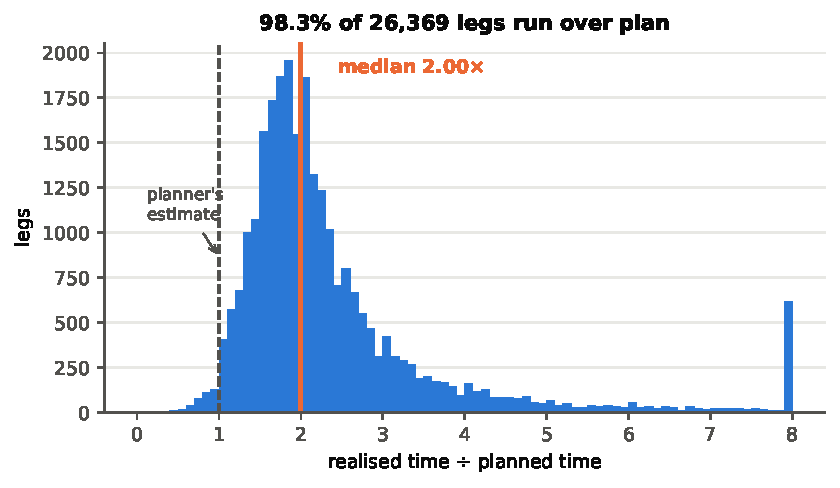
\includegraphics[width=0.88\columnwidth]{fig1_gap_ratio_distribution.pdf}
\caption{Distribution of realised over recorded planned time across \fzLegsTotal{} legs (source: \texttt{benchmarks/raw/w1\_*}). The mass sits well to the right of 1.0: 98.3\% of legs run over the estimate and the median ratio is \fzMedianGapRatioDpOne{}.}
\label{fig:premise}
\end{figure}
\fi

\section{Related Work}\label{sec:related}

\textit{Route engines and residual prediction.} OSRM is an open-source routing engine over OpenStreetMap data~\cite{luxen2011real}; route engines estimate travel time from road-class speed profiles and have no notion of hub dwell or a corridor's history. DeeprETA~\cite{hu2022deepreta} post-processes a route planner's estimate with a learned residual at industrial scale, the same structure as ours; our aim differs in treating localisation of the planner's error as primary and in reporting by slice. Other learned travel-time estimators address urban trajectories~\cite{wang2018learning,wang2018deeptte,fang2020constgat,derrowpinion2021eta}; delivery-time and route prediction are surveyed by Wen et al.~\cite{wen2023survey} (a preprint), and boosting is a strong baseline for delivery times~\cite{khiari2020boosting}.

\textit{Freight travel-time reliability.} Transport research characterises corridors with descriptive indices such as the planning-time and buffer indices~\cite{fhwa2005reliability,jones2005measuring,margiotta2013shrp2} and percentile spreads or fitted distributions~\cite{monsere2009truck,figliozzi2012reliability,pu2011analytic,unnikrishnan2022statistical}. We share the unit of analysis and add multiplicity-controlled testing that respects dependence.

\textit{Multiple testing and shrinkage.} False discovery rate control~\cite{benjamini1995controlling}, its validity under dependence~\cite{benjamini2001control} and large-scale inference~\cite{efron2010large} frame the audit; permutation tests for clustered data~\cite{good2005permutation,phipson2010permutation} and cluster-robust inference~\cite{cameron2015practitioner} frame the dependence-aware variant. Empirical-Bayes ranking~\cite{efron1975data,morris1983parametric,laird1989empirical,gelman2007data,goldstein1996league} frames the shrinkage ranking.

\textit{Forecast evaluation and leakage.} We use the Diebold--Mariano comparison with a Newey--West variance~\cite{diebold1995comparing,harvey1997testing}, block resampling for dependent data~\cite{kunsch1989jackknife,politis1994stationary}, rolling-origin evaluation~\cite{tashman2000out,bergmeir2012use}, and treat leakage as a reproducibility threat~\cite{kaufman2012leakage,kapoor2023leakage}.

\textit{On this dataset.} Searches in September and October 2026 found notebooks and case studies on the Delhivery records, typically comparing actual and OSRM time, but no peer-reviewed study; this is a statement about the search, not about the world. With no published result to compare with, every result below is reported beside a trivial policy computed on the same data.

\subsection{Extended related work}\label{sec:related_ext}

\textit{Stream processing and serving.} Spark~\cite{zaharia2016apache,zaharia2012resilient} descends from the MapReduce model~\cite{dean2008mapreduce}; its structured-streaming engine~\cite{armbrust2018structured} and the Kafka log~\cite{kreps2011kafka} are the substrate of our replay, and MLlib~\cite{meng2016mllib} supplies the distributed boosting. Our contribution there is not a new engine but a measured equivalence: a stateful streaming job whose predictions equal batch predictions on every leg, and a note on what that test cannot catch (a leak in a join that both sides share).

\textit{Gradient boosting and tabular benchmarks.} Boosting~\cite{friedman2001greedy} remains a default for tabular targets, with efficient implementations~\cite{chen2016xgboost,ke2017lightgbm,prokhorenkova2018catboost}, and tree ensembles have been reported to remain competitive with deep models on medium-sized tabular data~\cite{grinsztajn2022why}; random forests~\cite{breiman2001random} were our weaker first champion. We compare libraries under an identical, small tuning budget and report the ones that tie, rather than a single winner.

\textit{Evaluation hygiene.} The two pitfalls we report belong to a larger literature on leakage and reproducibility in learned systems~\cite{kaufman2012leakage,kapoor2023leakage} and on reporting practice~\cite{pineau2021improving,arp2022dos}. Our pre-registration is internal and timestamped rather than external, which we state as a limit.

\textit{Choosing among models and comparing them.} Comparing many models on one dataset raises the multiplicity problems that rank-based tests address~\cite{demsar2006statistical}; with a single dataset and a single metric we use paired resampling and a forecast-comparison test instead, and take rolling-origin folds as the check on a single split~\cite{tashman2000out,bergmeir2012use,hyndman2006another}.

\textit{Language-model agents for operations.} Agents that interleave reasoning with tool calls~\cite{yao2023react,schick2023toolformer,wei2022chain} are surveyed as a field~\cite{wang2024survey,xi2023rise}; retrieval-grounded generation~\cite{lewis2020retrieval} and model-based judging~\cite{zheng2023judging} are common evaluation scaffolds, and we note that our groundedness judgements were made by one human reader. A standard protocol for exposing tools~\cite{mcp2025specification} lets agents reach our corridor data and the transport-management system; the nearest design is a language model that explains an optimiser's output while the optimiser decides~\cite{li2023optiguide}.

\textit{Control towers.} In supply-chain practice a control tower is a central point of visibility and coordination over shipments~\cite{trzuskawska2017control}; adjacent literature discusses supply-chain visibility and integration~\cite{barratt2007antecedents,somapa2018characterizing,francis2008supply,chaffin2024systematic}. Our system takes the name for the same role and contributes an evaluated prototype, not a deployed one.

\section{Data and Problem Definition}\label{sec:data}

\subsection{The records and what they are}
The raw records are 144,867 scan-level segments across 14,817 trips collected between 12 September and 8 October 2018. Cleaning repairs types and keys and flags 2,600 suspect segments without dropping a row. Segments are reconstructed into \fzLegsTotal{} origin--destination \emph{legs} on \fzCorridorsTotal{} \emph{corridors}, a corridor being an ordered pair of facilities; the legs touch 1,657 facilities (Table~\ref{tab:dataset}). A leg is one trip's movement from one facility to the next. No trip visits a corridor twice, so every tested corridor's legs come from distinct trips.

\begin{table}[t]
\caption{The dataset after reconstruction. Splits are chronological by leg creation time; the validation cut is the last fifth of the training legs.}
\label{tab:dataset}
\centering
\begin{tabular}{@{}lr@{}}
\toprule
Quantity & Value \\
\midrule
Raw scan segments / trips & 144,867 / 14,817 \\
Legs / corridors / facilities & \fzLegsTotal{} / \fzCorridorsTotal{} / 1,657 \\
Corridors with at least 10 legs (tested) & \fzCorridorsTested{} \\
Legs on tested corridors & \fzLegsCovered{} \\
Calendar days of leg creation (India time) & 22 \\
Training / validation / test legs & \fzSplitTrain{} (16,876 + 4,219) / \fzSplitTest{} \\
Test legs with no prior leg on the corridor (cold) & \fzColdLegsTest{} \\
Legs with no prior corridor history, all legs & 11.09\% \\
\bottomrule
\end{tabular}
\end{table}

\paragraph{What the planned time is, and what we cannot know.} The planned time is the dataset's \texttt{osrm\_time} column, with \texttt{osrm\_distance}; its name says it comes from OSRM, an open-source route planner, and the dataset documents nothing more. We call it ``the OSRM estimate recorded in the dataset''. We cannot know how or whether the carrier used it operationally, which OSRM version or speed profile produced it, or whether the carrier's own planning had access to corridor history. We therefore make no claim about the carrier's planning system; the error measured is that of this recorded estimate against realised time, directly and not by simulation.

\paragraph{Notation.} For leg $i$ on corridor $c(i)$ let $a_i$ be the realised moving time and $o_i$ the recorded OSRM time, both in minutes. The \emph{log ratio} is $r_i=\log(a_i/o_i)$ and the \emph{gap} is $g_i=a_i-o_i$. The corridor audit works with $r_i$, which makes comparisons multiplicative and symmetric; prediction works with $g_i$, because the metric is minutes.

\paragraph{Dwell is separated from movement.} Realised moving time excludes dwell at the hub, the scan-to-scan interval minus moving time. The median leg spends 49 minutes, 34.6\% of its wall clock, parked. A leg finishes at its final scan, not at departure plus moving time; an earlier version of our pipeline used the latter, placed finishes a median 49.6 minutes early and counted unfinished legs as history. A leg is called delayed when it exceeds twice its plan; at that threshold \fzPctDelayedDpOne{}\% of legs are delayed.

\subsection{As-of features}\label{sec:asof}
Every feature describing a corridor's or hub's history is computed only from legs that had \emph{finished} before the leg in question was \emph{created}, with completions ordered before creations on a tie (Algorithm~\ref{alg:asof}). Legs with no prior leg on their corridor carry an explicit cold indicator rather than a zero that would read ``known to be on time''. Because a leakage rule is a claim, we verified it: an independent reconstruction of the as-of history agrees with the production implementation on every leg with history. Before the finish-time correction above the agreement was 95.2\%, which is how that error was found.

\begin{algorithm}[t]
\caption{As-of history for a query leg $q$ created at time $t_q$ (hierarchical back-off)}
\label{alg:asof}
\begin{algorithmic}[1]
\STATE $F \leftarrow \{\text{legs } j : \text{end}_j < t_q\}$ \hfill \COMMENT{facts first on ties}
\FOR{level $\ell$ in (corridor, origin hub, destination hub, route type $\times$ distance band, network)}
  \STATE $F_\ell \leftarrow \{j \in F : \text{key}_\ell(j)=\text{key}_\ell(q)\}$
  \IF{$F_\ell \neq \emptyset$}
    \STATE \textbf{return} level $\ell$, $n=|F_\ell|$, $\operatorname{median}\{g_j : j\in F_\ell\}$
  \ENDIF
\ENDFOR
\end{algorithmic}
\end{algorithm}

\section{The Corridor Audit}\label{sec:audit}

\subsection{Method}
For corridor $c$ with $n_c\ge 10$ legs let $\bar r_c$ be the mean log ratio and $\bar r_{-c}$ the mean over all other legs. The statistic is Welch's unequal-variance $t$~\cite{welch1947generalization},
\begin{equation}
t_c=\frac{\bar r_c-\bar r_{-c}}{\sqrt{s_c^2/n_c+s_{-c}^2/n_{-c}}},
\end{equation}
where the comparison group's sums come from subtracting the corridor's own from the network totals, so all \fzCorridorsTested{} tests need one pass over the data. The $p$-values are corrected for $m=\fzCorridorsTested{}$ tests by the Benjamini--Hochberg step-up procedure at level 0.05~\cite{benjamini1995controlling}, which controls the false discovery rate under independence or positive dependence, or by the Benjamini--Yekutieli procedure~\cite{benjamini2001control}, which is valid under arbitrary dependence at the price of the factor $\sum_{k\le m}1/k\approx 7.6$.

\paragraph{The independence assumption fails, and by how much.} Welch's test treats legs as independent. Before choosing a remedy we measured the dependence (the intraclass correlations are \ifjournal in Table~\ref{tab:dependence}\else 0.07 for a trip, under 0.01 for a day and \fzDepIccServiceCellDpTwo{} for a (corridor, service) cell\fi). Trips do not cluster a corridor's legs, because no trip visits a corridor twice, and the creation day is almost irrelevant. What clusters is the recurring \emph{service}: the same \texttt{route\_schedule\_uuid} repeats, \fzDepSingleServiceCorridors{} of the \fzCorridorsTested{} tested corridors run under exactly one service, and legs of one (corridor, service) cell are correlated (intraclass correlation \fzDepIccServiceCellDpTwo{}), giving a design effect of \fzDepDesignEffectMedianDpTwo{} at the median corridor: its 15 legs carry the information of about 7 independent ones. For those corridors a corridor effect and a service effect cannot be told apart.

\ifjournal
\begin{table}[t]
\caption{Dependence among the legs of tested corridors (source: \texttt{b3\_dependence\_diagnostics.json}).}
\label{tab:dependence}
\centering
\begin{tabular}{@{}lr@{}}
\toprule
Candidate cluster & Intraclass correlation \\
\midrule
Trip (legs of one trip, corridor-demeaned) & 0.072 \\
Creation day & \fzDepIccDayDpTwo{} \\
(Corridor, service) cell & \fzDepIccServiceCellDpTwo{} \\
\bottomrule
\end{tabular}
\end{table}
\fi

\paragraph{Cell permutation test.} The exchangeable unit is therefore the (corridor, service) cell. Let $\bar y_b$ and $m_b$ be a cell's mean log ratio and leg count. Cells are stratified by size (1 to 8 exactly, then 9--11, 12--15, 16--22, 23 and over) and one permutation shuffles the cell means among cells of the same stratum, each position keeping its own size and corridor. The permuted corridor statistic is the corridor's weighted mean of permuted cell means minus the mean of the rest, and the $p$-value is two-sided,
$p_c=(1+\#\{|D^{*}_c|\ge|D_c|\})/(B+1)$, with $B=100{,}000$ permutations~\cite{phipson2010permutation}. We report four variants on the same corridors: Welch or permutation $p$-values, each under BH or BY. A rule fixed in advance (decision D-080) names the \emph{headline} as the valid variant with the fewest significant slower corridors. We also measure the size of the standard test with a placebo: 200 datasets in which cell means are permuted among cells, destroying any corridor effect while keeping the cluster structure.

\subsection{Result}
\begin{table}[t]
\caption{Corridors significant at 5\% under four variants of the audit, of \fzCorridorsTested{} tested.}
\label{tab:variants}
\centering
\begin{tabular}{@{}lrr@{}}
\toprule
Variant & Slower & Faster \\
\midrule
Welch, BH (the original audit) & \fzBottlenecks{} & \fzFasterCorridors{} \\
Welch, BY & \fzAuditByWelchSlower{} & \fzAuditByWelchFaster{} \\
Cell permutation, BH & \fzAuditBhPermSlower{} & \fzAuditBhPermFaster{} \\
\textbf{Cell permutation, BY (headline)} & \textbf{\fzAuditRobustHeadlineSlower{}} & \textbf{\fzAuditRobustHeadlineFaster{}} \\
\bottomrule
\end{tabular}
\end{table}

The original procedure finds \fzBottlenecks{} corridors significantly slower and \fzFasterCorridors{} significantly faster than the network, covering 78.6\% of legs (\fzLegsCovered{} of \fzLegsTotal{}). Under Welch with BY these fall to \fzAuditByWelchSlower{} and \fzAuditByWelchFaster{}, which is the price of arbitrary dependence alone. Under the cell permutation the counts collapse (Table~\ref{tab:variants}). By the rule fixed in advance the headline is the cell permutation under BY, \textbf{\fzAuditRobustHeadlineSlower{} slower and \fzAuditRobustHeadlineFaster{} faster}, and so no corridor is \emph{robust} in our sense (significant under both the headline and the original); all \fzBottlenecks{} and \fzFasterCorridors{} original discoveries are \emph{fragile}.

\paragraph{The placebo explains why.} In the 200 placebo datasets, where corridor membership carries no information but services still differ, Welch rejects \fzAuditPlaceboRejectionPct{}\% of corridors uncorrected at the nominal 5\%, and Welch with BH finds on average \fzAuditPlaceboDiscoveriesDpOne{} ``significant'' corridors against 785 (\fzBottlenecks{} slower plus \fzFasterCorridors{} faster) on the real data. The standard test's false-positive load on this network is therefore large enough to account for most of what it reported.

\paragraph{What the strictest result does not say.} The headline is partly a property of the test's resolution. With $B=100{,}000$ the smallest attainable permutation $p$ is $1/(B+1)\approx 10^{-5}$, which is larger than the smallest BY threshold ($0.05/(1130\cdot 7.6)=5.8\times10^{-6}$), so that variant \emph{cannot} reject any corridor however large its effect, and BH needs $p\le 4.4\times 10^{-5}$ for its first rejection. The permutation $p$-values are not empty: \fzAuditPermPBelowFivePct{} corridors fall below 0.05 and \fzAuditPermPBelowOnePct{} below 0.01, and the top-20 slow corridors ranked by permutation $p$ overlap the Welch top-20 at Jaccard \fzAuditTopTwentyJaccardListDpTwo{}. Section~\ref{sec:stability} supplies the evidence that matters here: whether the corridor effects replicate. Our reading is that the \fzBottlenecks{} are a \emph{screening list}, not confirmed bottlenecks, and that the data cannot separate a corridor effect from a service effect for the corridors that run under one service.

\paragraph{What a zero means: a power study.} A zero is ambiguous between no effect and a test too weak to see one, so we measured the test. In the placebo world (real cell structure, cell means shuffled, no corridor effect anywhere) we planted a known shift of the log ratio into 30 corridors, 10 in each of three leg-count bins, and ran all four variants on 30 simulated datasets per shift; permutation $p$-values are exact down to $10^{-6}$ against a null bank checked against the real run (no corridor classified differently under BH or BY). The cell-permutation test is correctly sized (with no planted effect, \fzPowerPermSizeByPct{}\% of datasets show a BY rejection) and nearly blind: at a shift of 0.5, a 1.65-fold larger overrun, it finds \fzPowerByPermShiftHalfPct{}\% of planted corridors, and at a shift of 1.0, a 2.7-fold overrun, \fzPowerByPermShiftOnePct{}\% under BY and \fzPowerBhPermShiftOnePct{}\% under BH, rising to \fzPowerByPermLargeShiftOnePct{}\% for corridors with 25 or more legs and falling to \fzPowerByPermSmallShiftOnePct{}\% for 10 to 14 legs (Fig.~\ref{fig:power}). It never reaches 80% on the grid. The reason is the null itself: it mixes all cells of a size stratum, and real heterogeneity between services already spreads the cell means widely, so one corridor must stand far out. Welch fails in the other direction: it finds planted corridors easily, but at a shift of 0.5 \fzPowerWelchBhFdpShiftHalfPct{}\% of its discoveries are not planted corridors (nominal 5%), and with nothing planted it still rejects \fzPowerWelchBhRateShiftZeroPct{}\% of the corridors it was asked to find. So the zero says almost nothing about whether corridor effects exist, and it does show that the standard test's discoveries are mostly false; corridor effects rest on the stability result below, not on any single-corridor test.

\begin{figure}[t]
\centering
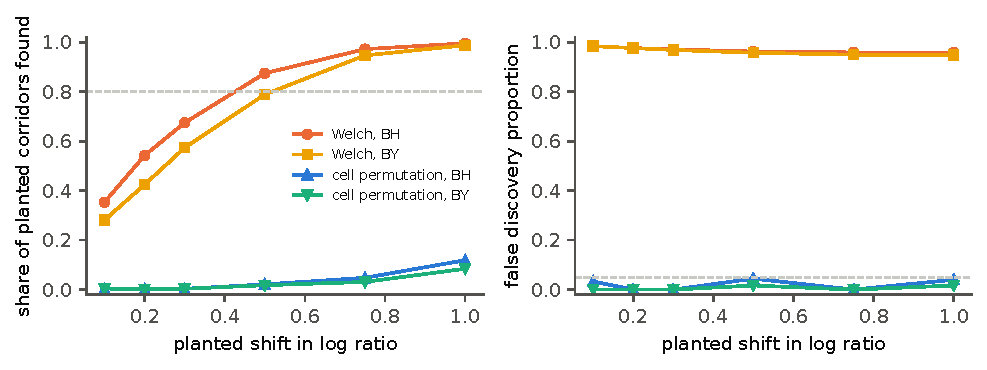
\includegraphics[width=\columnwidth]{fig_power_curves.pdf}
\caption{Simulated power (left) and false discovery proportion (right) of the four audit variants as a known shift is planted into 30 corridors of the placebo world; dashed lines mark 80\% power and the nominal 5\% (source: \texttt{b9\_power.json}).}
\label{fig:power}
\end{figure}

\subsection{Ranking corridors: shrinkage and the support floor}\label{sec:support}
A first version of this analysis found that raising the support floor from 10 to 30 legs changes the top-20 list completely, and proposed empirical-Bayes shrinkage as the remedy. We model the corridor means as $\hat\theta_c\sim N(\theta_c,v_c)$ with $\theta_c\sim N(\mu,\tau^2)$, estimate $\tau^2$ by REML (0.138, 0.133, 0.083, 0.058 at floors of 5, 10, 20 and 30 legs), and rank corridors by the posterior probability $P(\theta_c>t)$ that the corridor's true log ratio exceeds a material threshold $t=\fzEbThresholdLogDpTwo{}$ (a ratio of 3.27 to the recorded estimate)~\cite{efron1975data,morris1983parametric,laird1989empirical,gelman2007data}.

Pre-registered hypothesis: shrinkage removes the floor dependence. \textbf{It does not.} The corridors' own sampling variances (about 0.002) are small against $\tau^2$, so the median shrink factor is only 1\% to 2\% and the posterior mean is within a few percent of the raw mean. The ranking by probability is slightly more stable by our rule (mean pairwise top-20 Jaccard across the six floor pairs \fzEbTopTwentyJaccardEbDpTwo{} against \fzEbTopTwentyJaccardRawDpTwo{}, bootstrap interval for the difference [\fzEbDiffCiLowDpTwo{}, \fzEbDiffCiHighDpTwo{}]), but both lists change almost completely: floors 5 and 30 share no top-20 corridor in either ranking. The cause is eligibility, not noise: rank positions of corridors present at both floors correlate at 0.9997 or more, and a lower floor admits small corridors with extreme means (mean top-20 corridor size 10.8 legs at floor 5, 47.7 at floor 30). At floor 10, \fzEbPExceedHalf{} corridors have $P(\theta_c>t)\ge 0.5$, \fzEbPExceedNine{} have 0.9 or more and \fzEbIntervalAbove{} have a 90\% interval wholly above $t$, so there are more material corridors than twenty slots. A heavy-tailed prior does not change this: corridor effects are in fact heavy-tailed (a Student $t$ prior with \fzEbtBestNuFloorTenDpOne{} degrees of freedom beats the normal by \fzEbtLoglikGainFloorTenDpOne{} log-likelihood units at floor 10), but the $t$ ranking overlaps across floors exactly as the normal one does (\fzEbtTopTwentyJaccardDpTwo{}), and for the extreme corridors it shrinks less, not more (\fzEbtRetainedTDpTwo{} of the distance from the mean kept against \fzEbtRetainedNormalDpTwo{}). We therefore recommend reporting the whole ranking with intervals and stating the floor, rather than a top-20; shrinkage is better calibrated, not a cure\ifjournal{} (Fig.~\ref{fig:eb})\fi.

\ifjournal
\begin{figure}[t]
\centering
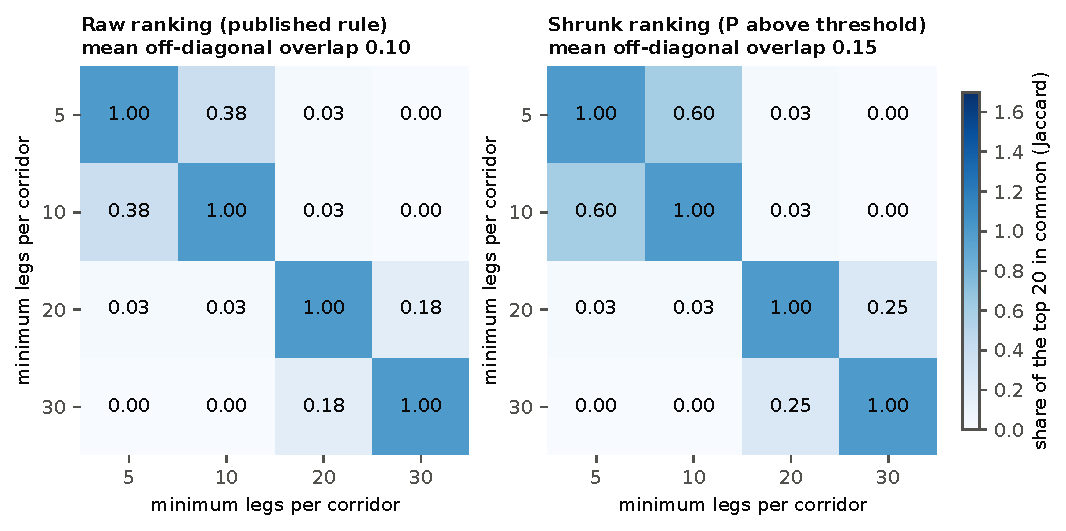
\includegraphics[width=0.85\columnwidth]{b4_eb_stability_heatmap.pdf}
\caption{Top-20 overlap between support floors for the raw and the empirical-Bayes rankings (source: \texttt{b4\_eb\_ranking.json}). Neither ranking is stable across floors; the empirical-Bayes one is marginally less unstable.}
\label{fig:eb}
\end{figure}
\fi

\subsection{Do the corridor effects persist?}\label{sec:stability}
We split the creation dates into two halves (12 and 11 dates), run the audit separately in each, and compare. The comparison universe is the \fzStabilityUniverse{} corridors testable in both halves at a floor of five legs per half. The raw corridor means correlate across halves at $\rho=\fzStabilitySpearmanDpTwo{}$. The slower sets of the two halves (Welch, BH) share Jaccard \fzStabilityJaccardDpTwo{} of their members against about 32 corridors expected by chance (hypergeometric $p<10^{-80}$), and \fzStabilityStillSlowerPct{}\% of the first half's slower corridors are also slower than the network in the second half, against a base rate of \fzStabilityBaseRatePct{}\% of corridors that are slower in the second half. By contrast the cell-permutation test with BY control finds nothing in either half or in any third. The two facts fit together: the pattern is persistent, but a corridor effect is not distinguishable from a service effect, and the same recurring services run in both halves, so persistence is not independent replication. The period is 22 calendar days of one season; Section~\ref{sec:threats} lists this among the limits.

\paragraph{Standard reliability indices.} The planning time index (95th percentile of travel time over free-flow time) and the buffer index are the usual descriptors of freight corridors\cite{fhwa2005reliability,jones2005measuring}. On the ratio scale, with the recorded OSRM time as free-flow time, the planning time index tracks the audit's mean log ratio closely (Spearman \fzIdxSpearmanPtiVsMeanDpTwo{}) and the buffer index does not (\fzIdxSpearmanBiVsMeanDpTwo{}). Between the two halves of the period the mean log ratio is the most stable descriptor (\fzIdxStabMeanDpTwo{}), the planning time index less so (\fzIdxStabPtiDpTwo{}, interval [\fzIdxStabPtiCiLowDpTwo{}, \fzIdxStabPtiCiHighDpTwo{}]) and the buffer index least (\fzIdxStabBiDpTwo{}, [\fzIdxStabBiCiLowDpTwo{}, \fzIdxStabBiCiHighDpTwo{}]); the intervals separate. A 95th percentile of 10 to 15 legs is a noisy statistic, so the standard indices add nothing that the mean does not carry here, and the buffer index is a poor ranking at this sample size.

\section{Predicting the Gap}\label{sec:prediction}

\subsection{Setup and the bar}
The quantity predicted is the gap $g_i$: how many minutes past its plan a leg will run, known when the leg is created. The split is chronological (\fzSplitTrain{} training legs and the latest \fzSplitTest{} for test) because a random split would score a model on legs interleaved in time with its training data. The metric is mean absolute error (MAE) in minutes, which the median minimises, so the comparator is an as-of \emph{median}, not a mean; using the per-corridor mean as the bar would have flattered every model by 3.1 minutes (\fzMaeCorridorMean{} against \fzBarOldMedianMaeDpTwo{}).

\paragraph{A bar without an unfair fallback.} The per-corridor median we first used as the bar predicts 0.0 minutes on a corridor with no history, that is, ``exactly on plan'', which is the OSRM estimate the whole paper shows to be wrong. Most of a model's margin sits on exactly those legs, so a reviewer can fairly say the baseline is handicapped. We therefore fixed, before measuring, a hierarchy of as-of medians (Algorithm~\ref{alg:asof}): the corridor; failing that the origin hub's outbound legs; the destination hub's inbound legs; the route type and distance band; the network. A shrunken variant weights each level by $n/(n+k)$. The bar is the baseline with the lowest test MAE of the three, which can only make the comparison harder for the model. The hard back-off scores \fzBarBackoffMaeDpTwo{} against \fzBarOldMedianMaeDpTwo{} for the old median and \fzBarShrunkMaeDpTwo{} for the shrunken variant (the best $k=1$; larger $k$ is monotonically worse), and is the bar. It is not harder on warm legs (identical to the old median there by construction); on the \fzColdLegsTest{} cold test legs it scores \fzColdMaeBackoffDpOne{} against 149.8.

\subsection{Models}
The target is the gap minus the baseline, and the prediction adds the baseline back, so a model that learns nothing reproduces the baseline. The 38 inputs are the leg's planned time and distance, departure hour, day and route type; as-of history for the corridor and both hubs with cold indicators; and corridor dispersion (median, 90th percentile, interquartile range, standard deviation), a trailing seven-day mean and hub dwell by part of day. We fit two families under the same budget (200 trees, depth 6, absolute loss, one learning rate chosen on a validation cut inside the training split, refit on all training legs, scored once on test). The distributed family is Spark MLlib gradient boosting~\cite{friedman2001greedy,meng2016mllib}, which the streaming and serving path \streamsec{} uses; the single-node family is LightGBM~\cite{ke2017lightgbm} with L1 loss, XGBoost~\cite{chen2016xgboost}, a histogram gradient-boosted regressor, a Huber-loss variant and a linear median regression. \emph{The reported model is whichever candidate has the lowest validation MAE, whatever library it comes from}; this rule was fixed in advance (D-077).

\begin{table}[t]
\caption{Test MAE on \fzSplitTest{} legs, with day-block bootstrap 95\% intervals. Validation MAE is the selection criterion. The \emph{served} model is what the streaming job and public API run.}
\label{tab:mae}
\centering
\begin{tabular}{@{}lrr@{}}
\toprule
Model & Validation & Test \\
\midrule
OSRM plan (context) & --- & \fzMaeOsrm{} \\
Per-corridor mean & --- & \fzMaeCorridorMean{} \\
Old median (0.0 cold fallback) & 29.89 & \fzBarOldMedianMaeDpTwo{} \\
\textbf{Hard back-off (the bar)} & \fzBarBackoffValidationMaeDpTwo{} & \textbf{\fzBarBackoffMaeDpTwo{}} \\
Spark GBT over the old median (served) & \fzVTwoValidationMaeDpTwo{} & \fzServedMaeDpTwo{} [\fzServedMaeCiLowDpOne{}, \fzServedMaeCiHighDpOne{}] \\
Spark GBT over back-off & \fzVThreeValidationMaeDpTwo{} & \fzVThreeTestMaeDpTwo{} \\
Linear median regression & 34.32 & \fzZooLinearMaeDpTwo{} \\
XGBoost, L1 & 28.00 & \fzZooXgboostMaeDpTwo{} \\
Histogram GBT, L1 & 27.54 & \fzZooHistgbrMaeDpTwo{} \\
LightGBM, Huber & 27.88 & \fzZooLightgbmHuberMaeDpTwo{} \\
\textbf{LightGBM, L1 (reported)} & \fzReportedValidationMaeDpTwo{} & \textbf{\fzReportedMaeDpTwo{}} [\fzReportedMaeCiLowDpOne{}, \fzReportedMaeCiHighDpOne{}] \\
\bottomrule
\end{tabular}
\end{table}

\subsection{Results with intervals}
Table~\ref{tab:mae} is the headline. The reported model scores \fzReportedMaeDpTwo{} against the bar's \fzBarBackoffMaeDpTwo{}: a difference of \fzReportedVsBarDeltaDpTwo{} minutes, with a day-block bootstrap 95\% interval of [\fzReportedVsBarCiLowDpTwo{}, \fzReportedVsBarCiHighDpTwo{}] that excludes zero, and it wins on all \fzSlicesTotal{} slices of the slice table (Fig.~\ref{fig:forest}). The served Spark model is behind it, at \fzServedMaeDpTwo{}, a difference to the bar of \fzServedVsBarDeltaDpTwo{} [\fzServedVsBarCiLowDpTwo{}, \fzServedVsBarCiHighDpTwo{}], winning \fzServedSlicesWon{} of the \fzSlicesTotal{} slices. We therefore report two models and say which is which: the reported model is single-node, the served one is the better Spark candidate by validation, and the paper does not claim they are the same model. Three independent boosting libraries land within 0.1 minute of one another over the old median (29.66, 29.71, 29.75), so the earlier single-node figure of 29.52 was not a lucky seed and the distributed model's \fzServedMaeDpTwo{} is simply behind the same recipe.

\paragraph{Three readings of the intervals, none flattering to a naive test.} Test legs are not independent: legs on one day share conditions. Our interval resamples whole India-time calendar days (six blocks), which is the most conservative of the three we compute; a six-hour-block bootstrap is narrower and a paired-leg bootstrap narrower still and optimistic. The Diebold--Mariano test~\cite{diebold1995comparing,harvey1997testing} with a Newey--West bandwidth of one day of legs agrees with the day-block conclusion for the reported model. Six blocks is few; the interval is honest about that but should not be over-read.

\begin{figure}[t]
\centering
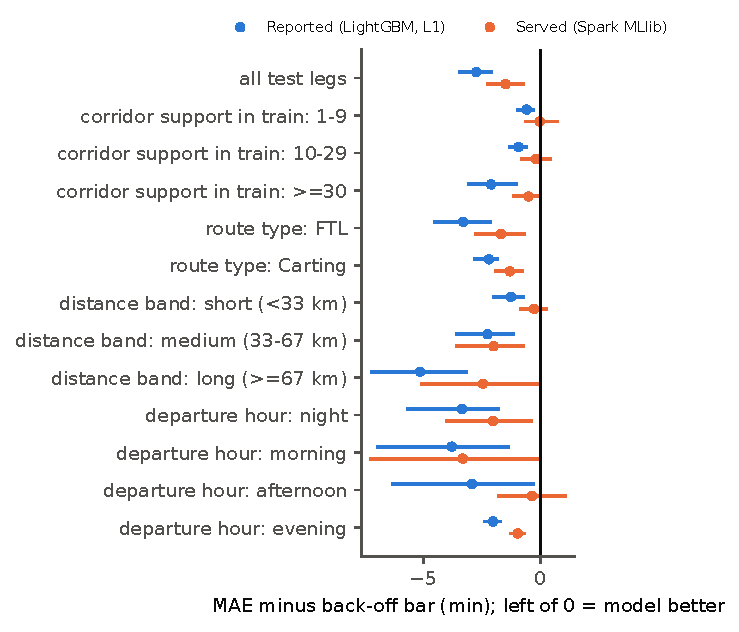
\includegraphics[width=0.78\columnwidth]{fig_forest_delta_mae.pdf}
\caption{MAE minus the back-off bar by slice, for the reported (LightGBM) and served (Spark) models, with day-block 95\% intervals (source: \texttt{b2\_significance.json}). The corridors unseen in training (a gain of about $-32$ minutes) are omitted to keep the scale readable.}
\label{fig:forest}
\end{figure}

\paragraph{Where the gain is.} Against the bar, the reported model's whole margin is concentrated on legs the bar has no history for. On the \fzColdLegsTest{} cold legs it scores \fzReportedColdMaeDpOne{} against the bar's \fzColdMaeBackoffDpOne{} (a difference of \fzReportedColdDeltaDpOne{} minutes, day-block interval [\fzReportedColdCiLowDpOne{}, \fzReportedColdCiHighDpOne{}]); on the warm legs the difference is \fzReportedWarmDeltaDpTwo{} minutes [\fzReportedWarmCiLowDpTwo{}, \fzReportedWarmCiHighDpTwo{}]. A back-off hierarchy is a strong lookup, and the model's value is mostly where a lookup has little to say. A note on validation: the validation cut did not favour the model over the bar (the bar scores \fzBarBackoffValidationMaeDpTwo{} there against the served model's \fzVTwoValidationMaeDpTwo{}), although the reported model does (\fzReportedValidationMaeDpTwo{}). We report both because the selection rule uses validation and the claim uses test.

\paragraph{Feature groups.} Removing one group at a time from the LightGBM model and measuring the change in test MAE with day-block intervals shows that only three groups carry detectable weight: the time of day and week (+\fzAblationTimeDeltaDpTwo{} minutes), the hub histories (+\fzAblationHubDeltaDpTwo{}) and the dispersion and dwell block (+\fzAblationDispersionDeltaDpTwo{}). Corridor history alone is redundant given the others ($\Delta=\fzAblationCorridorDeltaDpTwo{}$, interval including zero), which agrees with the gain sitting on cold legs.

\subsection{Rolling-origin check}\label{sec:rolling}
A single chronological split can be lucky. We therefore refit on four expanding windows of the 22 India-time calendar days (train through day 10, 13, 16 and 19; test on the next three days), with every hyperparameter frozen at its headline-split value and the baselines recomputed from each fold's training legs (pre-registered as D-076 and D-098). The reported model beats the back-off bar in \fzRoZooBeatsBarFolds{} of \fzRoFolds{} folds, by \fzRoZooDeltaMeanDpTwo{} minutes on average (standard deviation \fzRoZooDeltaSdDpTwo{} over folds), so the headline split's difference is not an outlier (Fig.~\ref{fig:rolling}). Each fold has only three days of test legs and none has an interval of its own.

The served Spark model does not fare as well. It beats the bar in only \fzRoServedBeatsBarFolds{} of the \fzRoFolds{} folds (mean difference \fzRoServedDeltaMeanDpTwo{} minutes, standard deviation \fzRoServedDeltaSdDpTwo{} over folds), so the headline split's \fzServedVsBarDeltaDpTwo{} is not robust to the choice of window, and the Spark model over the back-off baseline wins in \fzRoVThreeBeatsBarFolds{}. What does hold across folds is the cold-leg gain (mean cold-leg MAE \fzRoColdServedMaeDpOne{} against the bar's \fzRoColdBarMaeDpOne{}) and the bar itself: the back-off baseline beats the old median in every fold (\fzRoBarVsOldDeltaMeanDpTwo{} minutes on average). We therefore describe the served model as no worse than the bar and better on cold legs, not as better overall.


\begin{figure}[t]
\centering
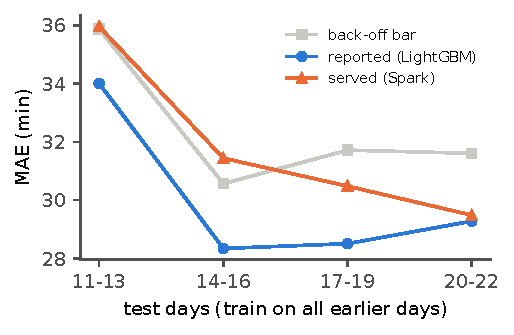
\includegraphics[width=0.6\columnwidth]{fig_rolling_origin.pdf}
\caption{MAE by rolling-origin fold: the back-off bar, the reported single-node model and the served Spark model (sources: \texttt{b2\_rolling\_origin\_zoo.json}, \texttt{b2\_rolling\_origin.json}).}
\label{fig:rolling}
\end{figure}


\section{Streaming and Serving}\label{sec:stream}

A producer replays legs as two kinds of event, a \emph{query} when a leg is created and a \emph{fact} when it finishes, and a structured-streaming job~\cite{armbrust2018structured} scores each query and raises an alert when the prediction crosses twice the planned time. Events travel through Kafka~\cite{kreps2011kafka} or a file source, and the model is a Spark MLlib ensemble~\cite{meng2016mllib}. Several features cannot be served from a static lookup: the seven-day window moves with each query, and dwell is keyed by hub and by the query's own part of the day. The job therefore keeps every corridor's and hub's history as \textbf{event-time state}: each fact updates the state of the keys it belongs to, each query reads that state as of its own time, and the state is persisted so that a restarted job resumes with the history it had. The updates repeat the batch arithmetic in the same order, so results are equal rather than close.

\paragraph{Equivalence.} Over the full \fzStreamEvents{}-event replay, run in two halves across a restart from the persisted state, \textbf{\fzStreamAllLegsIdentical{} of \fzStreamAllLegs{} legs score bit-identically to batch} (largest difference \fzStreamMaxAbsDifference{} minutes), and no history feature differs on any leg. The stream's own test-split predictions give the served model's \fzServedMaeDpTwo{} minutes. Replaying 2,000 legs through a live broker and through a file source produces the same alerts on the same legs with the same predicted gaps. The streamed model is the \emph{served} model (Section~\ref{sec:prediction}); the reported single-node model has not been put through this chain.

\paragraph{Throughput.} With a stateless history lookup the producer sustained \fzStreamProducedEpsDpOne{} events/s and the job scored \fzStreamScoringEpsDpOne{} events/s, with event-to-alert latency of \fzStreamLatencyPFiveZeroSDpOne{} s at the median on one 20-core machine. Event-time state costs throughput: the stateful job scored 74 events/s of busy time on the same machine, ample for the real event rate and too slow for a one-minute replay of three weeks. A public interface serves the same model with a tree evaluator identical to the distributed one on every leg, at \fzApiPNineFiveMsDpOne{} ms at the 95th percentile from a free-tier host.

\paragraph{Alerting is a workload decision.} For the best classifier, raising the delay threshold from $1.15\times$ to $2.0\times$ moves the Matthews correlation~\cite{matthews1975comparison,chicco2020advantages} only from 0.507 to 0.536, while the share of legs alerted falls from 98\% to 49\% (Fig.~\ref{fig:threshold}). The threshold is a policy about how many alerts an operator can act on, not a dial for quality.

\begin{figure}[t]
\centering
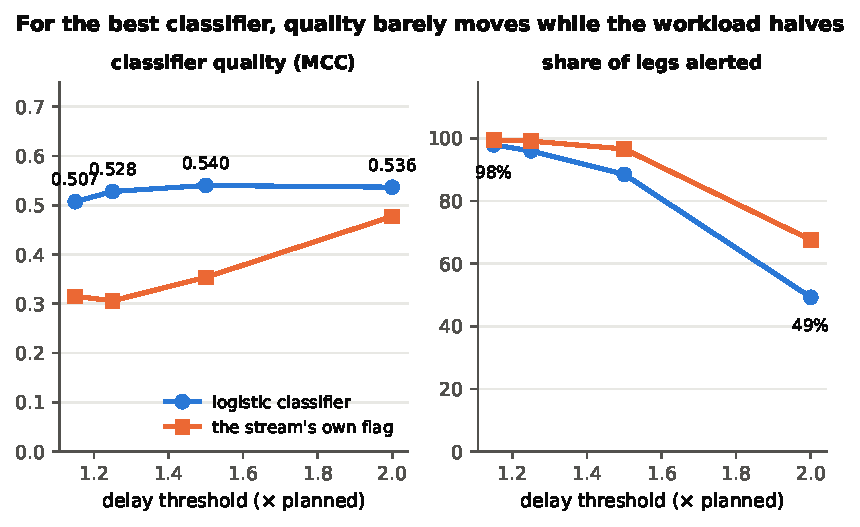
\includegraphics[width=0.88\columnwidth]{fig7_threshold_sensitivity.pdf}
\caption{Matthews correlation and alert volume across delay thresholds. Quality is nearly flat; workload is not.}
\label{fig:threshold}
\end{figure}

\section{Scale}\label{sec:scale}

The audit's two aggregation functions, imported unchanged, were run on New York City taxi trip records mapped into the leg shape; the planned time there is a stated stand-in, and no gap statistic is reported from those data. \textbf{\fzScaleRows{} rows aggregate in \fzScaleWallSDpTwo{}\,s on 20 cores}, \fzScaleRowsPerS{} rows per second (Fig.~\ref{fig:scale}). Two readings are unflattering and belong here: at this project's own size the runtime is the engine's fixed cost (\fzLegsTotal{} legs and 2.9 million trips both take 2.4\,s), and cutting the cores from 20 to 4 costs only \fzScaleWallSFourCoresDpTwo{}\,s against \fzScaleWallSDpTwo{}\,s, because reading 914\,MB from one disk is IO-bound. The scale run demonstrates that the aggregation scales; it does not show that the dependence-aware audit does, which has a permutation loop and runs in about a minute at $10^{5}$ permutations on this network.

\begin{figure}[t]
\centering
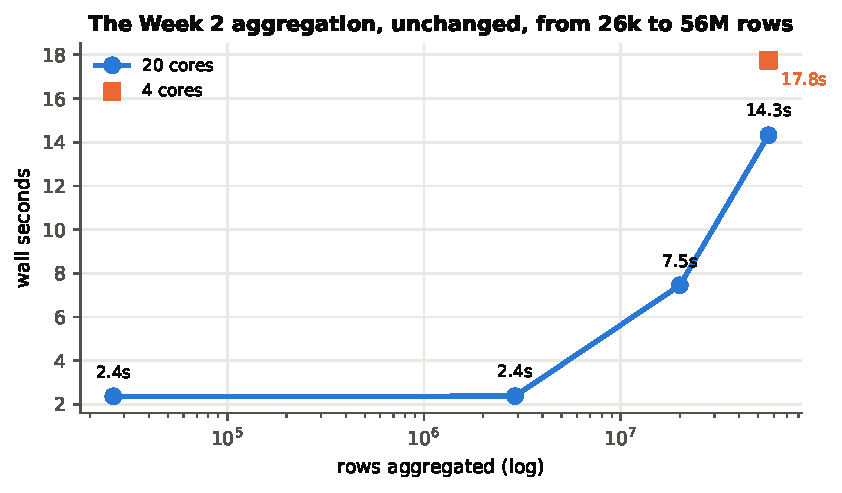
\includegraphics[width=0.88\columnwidth]{fig8_scale_runtime.pdf}
\caption{Aggregation runtime against input size and core count (source: \texttt{w7\_scale\_benchmark.json}).}
\label{fig:scale}
\end{figure}

\section{The Agent Layer as a Design Position}\label{sec:agents}

\subsection{Verdicts computed, prose generated}
Five agents (document extraction, order entry, exception triage, invoice audit and an analytics assistant) share one rule: every verdict is computed, and a language model writes only the sentence a person reads. Severity is arithmetic over how far past its threshold a leg is predicted to run; an invoice verdict is four comparisons. The rule makes each decision reproducible and therefore scorable, and bounds what a model error can do to a sentence. It follows the division of labour of systems in which a language model explains an optimiser's output while the optimiser decides~\cite{li2023optiguide}, applied more strictly, and builds on tool-using agent designs~\cite{yao2023react,wang2024survey,xi2023rise} exposed through a standard protocol~\cite{mcp2025specification}. Each agent's evaluation set was authored by someone other than its builder, and every result is reported beside a trivial policy on the same set. All agent data are synthetic or generated for this study; only the network data are real.

\paragraph{Scale re-runs.} First sets of 20 to 50 cases give perfect scores that are consistent with a true rate of 84\%, so the agents were re-run at scale, stratified so that hard cases form a named share, with Wilson intervals~\cite{wilson1927probable,agresti1998approximate}. Order entry scored \textbf{\fzOrderEvalScaleHeldoutPct{}\% on \fzOrderEvalScaleCases{} held-out emails} (95\% interval [79.4, 89.3]), falling to \fzOrderEvalScaleAdversarialHeldoutPct{}\% on the adversarial half, where every error was an order filed on a value the email never stated. Invoice audit was correct on \textbf{\fzInvoiceEvalScaleAccuracyPct{}\% of \fzInvoiceEvalScaleCases{} invoices} (interval [85.1, 93.4]) with \fzInvoiceEvalScaleFalseDisputes{} correct invoices disputed; its misses are the one kind that falls inside its own tolerance. The orchestrator routed \textbf{\fzLifecycleEvalScaleRoutingPct{}\% of \fzLifecycleEvalScaleCases{} lifecycles} as the email deserved, exercising all \fzLifecycleEvalScalePaths{} paths of its graph. Document extraction scored \fzDocExtractionAccuracyPct{}\% of fields on \fzDocExtractionRows{} of 40 planned rows (the remaining rows were not run for quota reasons). The assistant routed \fzAssistantRouteAccuracyLlmPct{}\% of 30 questions correctly with model phrasing and \fzAssistantRouteAccuracyPct{}\% without.

\paragraph{The 100\% on the 200-email set is not held out.} The rule-based order agent was fixed after the 200-email set found its first failures, so its later 100\% on that set is a fitted score. We therefore built a new held-out hard set (\fzHardOrderCases{} emails over hard templates such as Hinglish quantities, conflicting figures and quoted threads) and scored the \emph{unmodified} agents once: the order agent scored \textbf{\fzHardOrderRulesPct{}\%}, failing three template classes outright; the invoice auditor scored \fzHardInvoiceRulesPct{}\% on a boundary set. We did not repair the order failures, which are documented.

\subsection{Exception precision with uncertainty}\label{sec:exception}
Section~\ref{sec:replay} gives the as-of precision. The comparison with alerting on every leg is the one the replay's first version exaggerated: the corrected gain is \fzExcGainPointsDpTwo{} points, significant under the valid paired test, and the lowest severity grade performs worse than alerting everything.

\subsection{What the language model adds: a pilot ablation}\label{sec:ablation}
The design position makes a direct question answerable: what does each agent gain or lose when a model makes the decision itself? We ran the order agent with an open 120-billion-parameter model deciding, five sampled runs per case plus two at temperature zero, on the same stratified cases the rules saw. \emph{This is a pilot}: the free-tier daily token cap bound before the pre-registered 40 cases per agent, so the sample is \fzAblationOrderCases{} order cases (and 8 each for invoice and exception triage), a second small model at 8 each is reported separately, and the full design is resumable but not run. On those cases the rules scored 100\% (not held out, see above) and the model deciding scored \fzAblationOrderLlmAccuracyPct{}\% pooled over five runs (95\% interval [\fzAblationOrderLlmCiLowPct{}, \fzAblationOrderLlmCiHighPct{}]); the interval of the difference to the rules excludes zero. The model was less reproducible (all five runs agreed on \fzAblationOrderUnanimityPct{}\% of cases; Fleiss $\kappa=\fzAblationOrderKappaDpTwo{}$~\cite{fleiss1971measuring}) and filed 12\% of its orders on values the email did not state, against none for the rules. On invoice audit and severity grading, where the policy is arithmetic and given in the prompt, the pilot found no difference at $n=8$. The honest summary is that the evidence supports ``comparable where the policy is arithmetic'' and ``worse where it needs reading'' for the order task on this sample, and does not support the stronger claim that a deterministic core is generally better or cheaper: cost on a paid tier would be about a quarter of a dollar per thousand verdicts at assumed list prices that we did not verify, and latency is seconds against microseconds. The empty column of the study is human labels: no agent decision has been compared against a second labeller, and the protocol and sheets for that are prepared but not run.

\section{Two Evaluation Pitfalls}\label{sec:pitfalls}

\subsection{An optimiser setting that disabled the loss}\label{sec:optimiser}
Our first distributed residual model used absolute-loss boosting at a step size of 0.05 and reached 32.52 minutes, clearing the then bar by 1.6\% while losing to it on every corridor with history; its whole margin came from 294 legs on unseen corridors. Reading the saved model explained it. The library's absolute-loss boosting fits its first tree to the raw target with squared error (leaf values from $-1{,}382$ to $+2{,}605$ minutes) and every later tree to the \emph{sign} of the error, with leaf values in $[-1,1]$ scaled by the step size. At 0.05 the 199 corrective trees can move a prediction by at most 9.95 minutes in total, so the loss the model was chosen for was barely switched on. Validation over step sizes $\{0.05,0.3,1.0\}$, with correction caps of 9.95, 59.7 and 199 minutes, confirmed the mechanism in the ordering of the results, and 1.0 was chosen on validation. The general lesson: when a loss is chosen to match the metric, check that the optimiser can reach it; a default can silently cap the effect.

\subsection{A replay that scored the past with the future}\label{sec:replay}
The exception agent grades each predicted delay and alerts on it. Its notification precision was first measured at 72.1\% against 54.1\% for alerting on every leg. The measurement replayed the earliest 2,000 legs through a version of the streaming job that joined each query to the latest history snapshot: live, that is history up to now; in a replay it is history up to the end of the data. Of the 2,000 replayed legs, 1,290 had no corridor history at their own creation time and were scored as if they had fourteen prior legs. With only the history each leg had at its own time the precision is \textbf{\fzExcPrecisionAsOfRatePct{}\%} (Wilson 95\% interval [\fzExcPrecisionCiLowPct{}, \fzExcPrecisionCiHighPct{}] on \fzExcAlerts{} alerts). The snapshot run reproduces the first measurement exactly, so the gap is the leak and nothing else.

Precision rises with severity (Fig.~\ref{fig:severity}; Cochran--Armitage trend test~\cite{cochran1954some,armitage1955tests}, $p<10^{-40}$), so the grade is a useful filter, but the lowest grade falls \emph{below} the alert-everything policy. The gain over alerting on every leg is \fzExcGainPointsDpTwo{} percentage points, not 18. Because the two policies overlap (the alerted legs are a subset of all legs), an independent two-proportion test is invalid; the valid test compares alerted with not-alerted legs ($z=\fzExcGainZDpTwo{}$, bootstrap 95\% interval of the gain [\fzExcGainCiLowPct{}, \fzExcGainCiHighPct{}] points). Legs share corridors, so these intervals are optimistic and we had no corridor identifiers in the counts file to cluster on. A replay is an evaluation only if every join inside it is as-of the event being replayed~\cite{kaufman2012leakage,kapoor2023leakage}.

\begin{figure}[t]
\centering
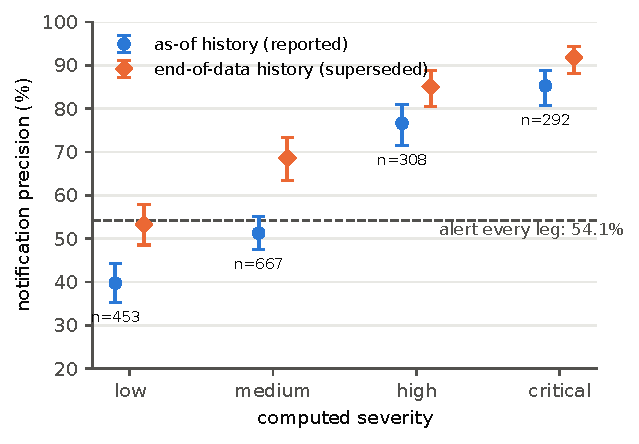
\includegraphics[width=\columnwidth]{fig_b8_severity_ci.pdf}
\caption{Notification precision by severity grade with Wilson 95\% intervals, as measured with as-of history, against the alert-every-leg policy (source: \texttt{b8\_exception\_stats.json}).}
\label{fig:severity}
\end{figure}

\section{Threats to Validity}\label{sec:threats}

\paragraph{Internal validity.} The cell-permutation test is a global-null permutation: with real corridor effects in the pool it is conservative for the strongest corridors, and it treats cells of one size stratum as equally noisy. Its strictest variant is resolution-limited at $10^{5}$ permutations (Section~\ref{sec:audit}); a ten-fold finer run, which rejects nothing either, is reported in the appendix of the journal version. Cells in different corridors that share a trip stay independent in the scheme, which BY control is meant to cover. The as-of rule prevents the leak we found in a streaming replay (Section~\ref{sec:replay}), but any further replay-based measurement inherits the risk. A leg created just before a rolling-origin window may finish inside it, so its label is not strictly known at the cut.

\paragraph{External validity.} One operator, one country and 22 calendar days of leg creation, in one season of 2018. Whether the corridors flagged persist over months or across carriers is untested; our persistence result is within the 22 days and the same recurring services run in both halves. The data record that a leg ran late, not why.

\paragraph{Construct validity.} The planned time is the dataset's recorded OSRM estimate; we cannot know the version, the profile or whether the carrier's own planning had corridor history, so the error measured is that of this recorded number and not of a production planner. A corridor is an ordered facility pair, which is not a physical road: two services on the same pair may take different roads.

\paragraph{Statistical conclusion validity.} Test legs span six calendar days, so the day-block interval rests on six blocks; the six-hour-block and Diebold--Mariano results agree for the reported model, but six blocks is few. One chronological split and four rolling folds (Section~\ref{sec:rolling}) are the evidence of stability. The validation cut favoured the bar over every Spark model while the test split favoured the models; the reported model was selected on validation by a rule fixed in advance, and both are shown. The 13 slices are not corrected for multiplicity in the figure; the headline claim uses the overall interval. The dependence-aware audit gives zero at its pre-registered strictness: this is a limit of what these data can confirm, not a proof that the corridors are null.

\paragraph{Evaluator and model choice.} The reported model is single-node and the served model is a distributed one; the paper does not claim they are the same. Hyperparameter search was identical in budget across libraries (three learning rates), so a larger search could change the ordering of the close candidates (29.66 to 29.75).

\section{Reproducibility, Ethics and Contributions}\label{sec:repro}

\paragraph{Reproducibility statement.} Every number in this paper is a \LaTeX{} macro generated by \texttt{python -m src.report.paper\_numbers} from \texttt{benchmarks/results\_freeze\_v6.json}, which records for each value the file it came from and that file's hash; \texttt{python -m src.ml.results\_freeze --verify} fails if a result file has changed since the freeze. A full rebuild from the raw CSV on a fresh clone took \fzFreshCloneRebuildS{} seconds on the reference machine (a 14-core, 20-thread Windows laptop) before the model-comparison and audit stages of this paper were added; with them the estimate, summed from per-stage timings and not re-measured as one run, is about six hours; the Spark stages need a local Hadoop shim on Windows, which the repository documents. Experiments that use randomness fix their seeds, and each was pre-registered as a dated, committed entry in \texttt{docs/decisions.md} before it was run; where we departed from a plan (the clustering unit in Section~\ref{sec:audit}, the reported model in Section~\ref{sec:prediction}) the departure is its own entry. The tracked tree holds no credentials, data or generated model files. A permanent archive with a DOI is a release step that the authors have prepared but not yet performed (see \texttt{HUMAN\_ACTIONS.md}).

\paragraph{Pre-registration and its limits.} Pre-registration here means a committed, timestamped decision entry that names the quantity, the rule and the reporting commitment before the run. It is a discipline against our own flexibility, not an external registry. Three amendments were made and are flagged: the tie-break for the audit's headline rule, the clustering unit, and the sensitivity run for the permutation test's resolution.

\paragraph{Ethics and data statement.} The trip records are public, contain no personal data, and are published on Kaggle under the dataset's own licence, which governs their use; we do not redistribute them. The agents' documents, emails and invoices are synthetic. No human subjects took part. The planned-time column is treated as the dataset's, and no claim is made about the carrier's operations.

\ifdefined\anonmode\paragraph{Author contributions (CRediT).} Withheld for review.\else
\paragraph{Author contributions (CRediT).} Following the repository's role split: K.\,S.\,K.\,Reddy, software and investigation for the agent layer, the dashboard and the orchestration; M.\,Lahari, methodology, software and validation for the models and their evaluation, and the reference review; S.\,M.\,Reddy, data curation, software and investigation for the data pipeline, the streaming path, the audit statistics and the deployment. All three authors wrote and reviewed the manuscript. \emph{Final author order and affiliations are a human decision and are placeholders here.}
\fi

\section{Conclusion}\label{sec:conclusion}

The OSRM estimate recorded in the Delhivery data errs one way almost always, and that error is real but harder to localise than a first analysis suggested. A standard Welch audit flags \fzBottlenecks{} slow and \fzFasterCorridors{} fast corridors, but on this network that procedure also reports about \fzAuditPlaceboDiscoveriesDpOne{} discoveries when corridor labels carry no information, and the cluster-aware test confirms none of them at its pre-registered strictness. The corridor effects nonetheless persist between halves of the period (rank correlation \fzStabilitySpearmanDpTwo{}), so the list is best read as a screening list whose members are real as patterns of recurring services and not yet as separable corridor effects. Empirical-Bayes ranking is a little better calibrated and no cure for the support floor. For prediction, a residual model over a fair back-off bar wins by \fzReportedVsBarDeltaDpTwo{} minutes with an interval that excludes zero, almost all of it where the bar has no history. Two findings concern evaluation rather than the network: an optimiser default that disabled the chosen loss, and a replay that leaked the future into alert scoring, which inflated a precision from 58.6\% to 72.1\%.

Future work: an audit over a longer period and several carriers, to separate corridor from service effects; a human-labelled comparison for the agent layer; and a live evaluation of alert precision.

\section*{Data and Code Availability}
The source data are public\footnote{Kaggle dataset ``Delhivery logistics dataset'' (user \texttt{devarajv88}); licence terms are in \texttt{DATA\_LICENSE.md} of the repository. We could not re-open the dataset page on the day of writing, so it is cited by this footnote and not in the bibliography.} and are not redistributed. All code, the decision log with every pre-registration, each result file behind a number here, a model card and a data card are at \url{https://github.com/krishna-2-005/Agentic-AI-Logistics-Control-Tower}; every number in this paper is a macro generated from a frozen results file (\texttt{benchmarks/results\_freeze\_v5.json}). An interactive version of the results is at \url{https://control-tower-mu-rouge.vercel.app}.

\section*{Use of AI Tools}
During the preparation of this work the authors used a generative AI assistant to help draft and edit text and code. The authors reviewed and edited all content, verified every number against the underlying result files and every reference against its source, and take full responsibility for the publication.
% Human action: adjust this statement to the chosen venue's policy before submission (see HUMAN_ACTIONS.md).

\appendix
\section{Supplementary Results}\label{app:supp}

\subsection{Feature-group ablation}
Table~\ref{tab:ablation_groups} gives the change in test MAE when a group of inputs is removed from the LightGBM model (day-block 95\% intervals; source: \texttt{b6\_feature\_ablation.json}). Groups whose interval includes zero are not distinguishable from no effect at this sample size.

\begin{table}[t]
\caption{Change in test MAE (minutes) on removing a feature group from the reported model. A positive value means the group helped.}
\label{tab:ablation_groups}
\centering
\begin{tabular}{@{}lrl@{}}
\toprule
Group removed & $\Delta$ MAE & Interval excludes 0 \\
\midrule
Time of day and week & \fzAblationTimeDeltaDpTwo{} & yes \\
Hub history & \fzAblationHubDeltaDpTwo{} & yes \\
Dispersion and dwell & \fzAblationDispersionDeltaDpTwo{} & yes \\
Corridor history & \fzAblationCorridorDeltaDpTwo{} & no \\
Plan and route; distance; baseline descriptors & $<0.07$ in size & no \\
\bottomrule
\end{tabular}
\end{table}

\subsection{Permutation-test resolution}
With $10^{5}$ permutations the smallest attainable $p$ is $10^{-5}$, above the smallest Benjamini--Yekutieli threshold, so the strictest variant could not reject anything. A ten-fold finer run ($10^{6}$ permutations, same seed and cells; pre-registered as D-084 before it was run) lowers the floor to $10^{-6}$, below that threshold, and still rejects nothing: \fzAuditFineByPermSlower{} slower corridors under BY and \fzAuditFineBhPermSlower{} under BH; the smallest permutation $p$ is $3.3\times10^{-5}$ (against $4.0\times10^{-5}$ at $10^{5}$), and \fzAuditFinePBelowFivePct{} corridors fall below 0.05. The headline is therefore not an artefact of resolution.


\subsection{Audit figures}
\begin{figure}[t]
\centering
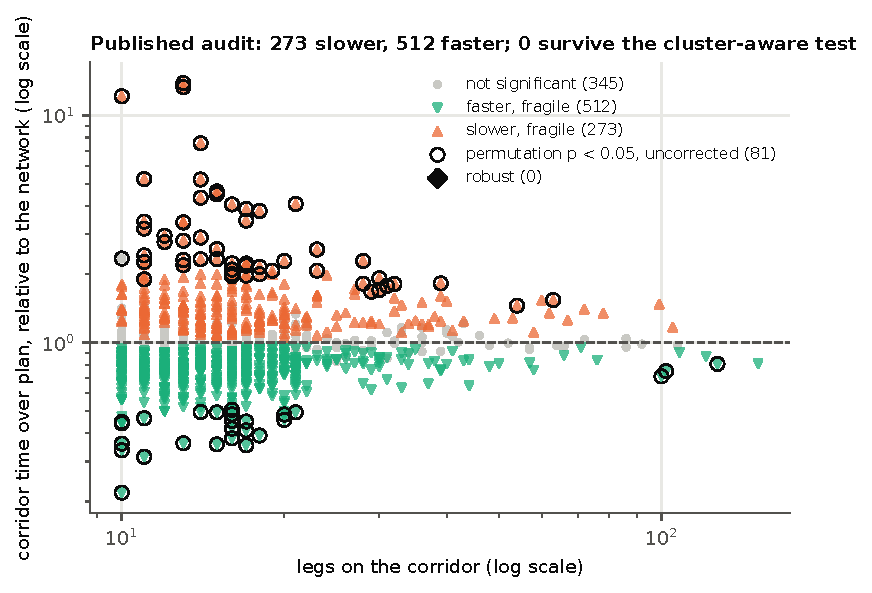
\includegraphics[width=\columnwidth]{b3_audit_robust.pdf}
\caption{Corridors by original and cluster-aware evidence (source: \texttt{b3\_audit\_robust.json}).}
\label{fig:b3}
\end{figure}

\begin{figure}[t]
\centering
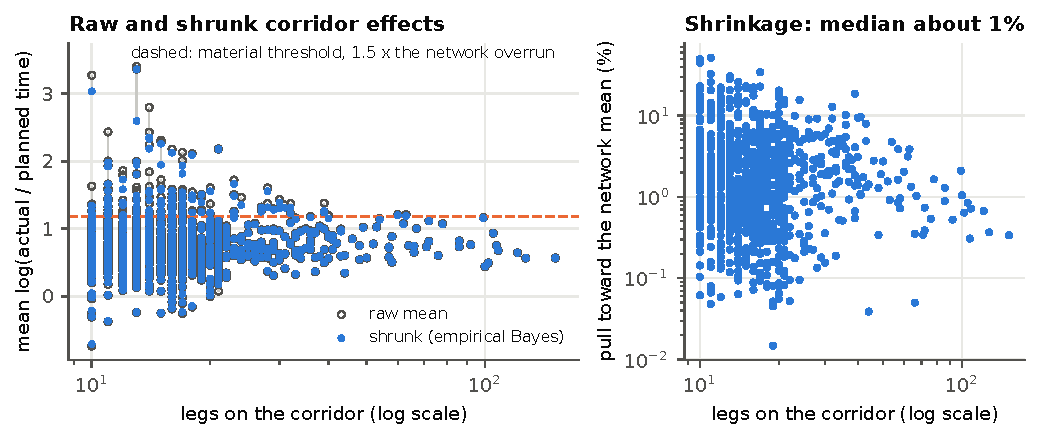
\includegraphics[width=\columnwidth]{b4_eb_shrinkage.pdf}
\caption{Empirical-Bayes posterior against raw corridor means: the shrinkage is small (source: \texttt{b4\_eb\_ranking.json}).}
\label{fig:b4}
\end{figure}

\begin{figure}[t]
\centering
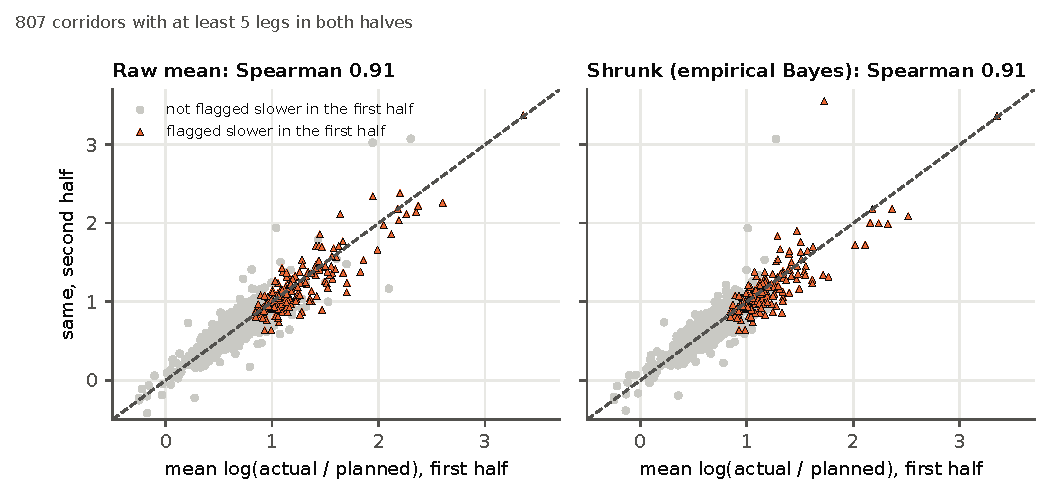
\includegraphics[width=\columnwidth]{b5_stability_scatter.pdf}
\caption{Corridor effects in the first half of the period against the second half (source: \texttt{b5\_stability.json}).}
\label{fig:b5}
\end{figure}

\begin{figure}[t]
\centering
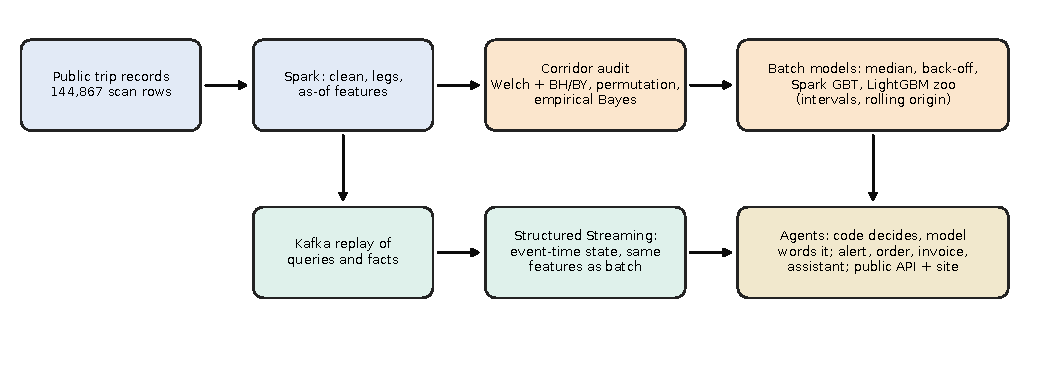
\includegraphics[width=\columnwidth]{fig_architecture.pdf}
\caption{System architecture: batch audit and models, streaming replay and serving, and the agent layer.}
\label{fig:arch}
\end{figure}


\bibliography{../refs_print}

\end{document}
